%\chapter{Designs}
%
%There are so many degrees of freedom in specifying a multi-touch interaction set that it would be a herculean feat to even just enumerate all of the potential designs. Thus, in this chapter, I will specify and evaluate only the three most distinct and representative multi-touch interaction set designs, which I have designated as the \emph{Closest Finger Design},  the \emph{Relative Indexing Design}, and the \emph{Absolute Indexing Design}. While it is quite likely that the ``optimal'' multi-touch interaction set design will  be a composition of these three designs, I will present each of them undiluted and unmixed in order to best highlight their individual characteristics.
%
%The Closest Finger Design, can best be thought of as a direct analogue to the Desktop Scratch mouse interaction set. In this design, sprites can only listen to one touch at a time, namely the presently closest touch. As a result of this one touch restriction, the set of touch blocks in the Closest Finger Design closely resemble the set of mouse blocks in Desktop Scratch.
%
%In contrast to the first design, the Relative Indexing Design enables sprites to listen to each of the up-to-ten simultaneous touches. Touch inputs in this design are indexed relative to the other concurrent touches in order of initiation from $1$ to the number of current touches. Note that since touches are indexed relatively in this design, a touch's associated index can  be subject to change. For example, a touch that was the third oldest current touch (meaning it has an associated index of 3) can become the oldest current touch (meaning an associated index of 1) if the two oldest current touches are lifted.
%
%Finally, like the previous design, the  Absolute Indexing Design also enables sprites to listen to each of the up-to-ten simultaneous touches. However, touches in this design are indexed in order of initiation relative to all touches that have made since the inception of the project, as opposed to just the current touches. As a result, a touch's associated index can never change in the Absolute Indexing Design, because the $n$th touch pressed in the execution of a project will forever be the $n$th touch pressed.


\chapter{Closest Finger Design}

As mentioned previously, one reason why programming multi-touch interactions can be so difficult is that there can be up-to-ten simultaneous touches on the tablet at any given moment. Thus, multi-touch input handling in Tablet Scratch can be significantly simplified, by restricting each sprite to only being able to listen to the touch closest to itself. This particular restriction is the main premise behind the \emph{Closest Finger Design}, the first of the three multi-touch interaction set designs that I will be presenting.

In this chapter (as will be the pattern for the two subsequent chapters), I will first specify the Closest Finger Design interaction set. Then, I will evaluate the design on the three iterations of case projects that I described in the previous chapter. However, at the end of this particular chapter, I will also present a possible extension that provides additional functionality to the interaction set design, but at the cost of simplicity and understandability.

\section{Interaction Set Specification}

The Closest Finger Design can best be thought of as a direct analogue to the Desktop Scratch mouse interaction set. In this design, sprites can only listen to one touch at a time, namely the closest touch at the moment of evaluation. As a result of this one touch restriction, the set of touch blocks in the Closest Finger Design closely resemble the set of mouse blocks that appear in Desktop Scratch.

In fact, the Closest Finger Design has a corresponding touch block for every mouse-related block in Desktop Scratch. While, the mouse blocks in a Desktop Scratch script are influenced by the status of the lone mouse,  the Closest Finger Design blocks in a sprite's scripts are, in general, similarly influenced by the status of the touch that is currently closest to that particular Sprite. 

There are (as of now) eight blocks in Desktop Scratch that are related to mouse inputs: five function blocks, two command blocks, and a single hat block. I will  present all of these blocks while also introducing and specifying their Closest Finger Design block counterparts.

\begin{figure}
\centering
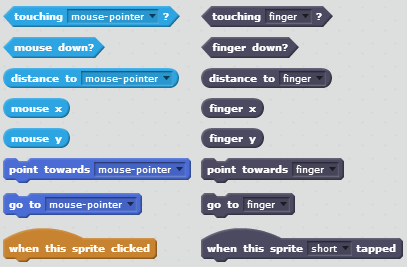
\includegraphics{images/Closest_Finger_Design_Block_Set.PNG}
\caption{Desktop Scratch's mouse interaction set with analogous Closest Finger Design blocks.}
\end{figure}

\subsection{Function Blocks}
The five mouse-related function blocks in Desktop Scratch are labeled ``touching mouse-pointer?", ``mouse down?", ``distance to mouse-pointer", ``mouse x", and ``mouse y". Following their namesakes, the ``touching mouse-pointer?" and ``mouse down?" blocks both produce Boolean values (e.g., \emph{true} or \emph{false}) corresponding to the current answer to their respective questions, while the ``distance to mouse-pointer", ``mouse x", and ``mouse y" blocks produce integer values (e.g., \emph{10}, \emph{-33}, \emph{147}, etc.) that similarly reflect their respective values. 

The first two equivalent Closest Finger Design function blocks, which I have labeled ``touching finger?" and ``finger pressed?", are relatively straight forward
\footnote{Note that these blocks reference ``fingers", but, in reality, most tablets cannot actually tell the difference between a touch coming from a finger or a touch coming from any other body part. However, for the sake of concreteness (and to avoid the potential confusion of a ``touch down" block), I have decided for blocks in the Closest Finger Design to refer to ``fingers" instead of ``touches".}.
As the name suggests, the ``touching finger?" block takes on a value of \emph{true} when a finger pressed on the tablet is touching the sprite using the block and a value of \emph{false} otherwise. Similarly, the ``finger pressed?" block takes on a value of \emph{true} when at least one finger is pressed on the stage and a value of \emph{false} when there are no touches.

The remaining three function blocks, labeled ``distance to finger", ``finger x", and ``finger y", are a little more difficult to articulate. In general, the ``distance to finger" block evaluates as the distance from the sprite to the touch that is currently closest to the sprite (i.e., the touch that has the shortest two dimensional distance to the center of the sprite with ties broken arbitrarily), while the ``finger x" and ``finger y" blocks represent the values of the latest x and y coordinates of that touch. When no fingers are currently being pressed on the tablet ``finger x" and ``finger y" will take the values corresponding to the location of last touch to have been made during the execution of the project. If the project just recently began and touches have yet to been made, ``finger x" and ``finger y" unfortunately must take on an arbitrary value. Since there is no ``null value" in Scratch and error messages are generally avoided, I have chosen for both ``finger x" and ``finger y" to evaluate to $0$ when no there are no prior touches. The ``distance to finger" block will always take the value of the distance between the current location of the sprite and the location with the coordinate values of ``finger x" and ``finger y".

\subsection{Command Blocks}
The two mouse-related command blocks in Desktop Scratch are the ``point towards mouse-pointer" and ``go to mouse-pointer" blocks, of which both when executed cause sprites to act as their names imply. Their equivalent Closest Finger Design blocks are similarly named ``point towards finger" and ``go to finger". Both of these blocks behave in a similar manner to their mouse counterparts, but focus on the location of the closest touch as opposed to that of the mouse.  

When there is at least one touch on the tablet, the location of interest for the blocks becomes that of the closest touch. Meanwhile, when no touches are currently present, the location of interest becomes the last location of the last touch. Finally, when no touches have been made during th execution of the project, the location of interest becomes the arbitrarily chosen coordinate of $\{0,0\}$.

To put it simply, executing the ``point towards finger" block cause sprites to point towards the location at the present coordinate values of ``finger x" and ``finger y". Similarly, executing the ``go to finger" block causes the sprite go to that same location. 

\subsection{Hat Block}
Finally, the sole hat block in Desktop Scratch's mouse interaction set is the ``when this sprite is clicked" block. When triggered, this hat block initiates the execution of its connected stack each time the sprite is clicked by the mouse. Here, a click is defined as pressing down on the mouse left button and quickly releasing. If the sprite is clicked a second time before the connected stack has finished its first execution, Scratch restarts the execution of the stack. Note that because of Scratch's thread-switching behavior, this can only happen when the stack contains loops or long ``wait blocks". 

The equivalent hat block for the Closest Finger Design is the ``when this sprite is tapped" block, which is triggered whenever a sprite is tapped. A sprite is said to be ``tapped" whenever a finger is pressed down on the sprite and quickly lifted. The ``when this sprite is tapped" block handles repeat triggerings in the same way as its mouse counterpart, i.e., by restarting the execution of the connected stack. Note that this hat block can be triggered by any touch, not just the closest touch, although in practice the triggering touch will almost always be the closest touch.

Since a variety of single-touch gestures, including swiping, long taps, and double taps, are common place in tablet applications, it may be beneficial to augment the ``when this sprite is tapped" block to support other common gestures. Adding support for more common single-touch gestures lowers the floors to implementing those interactions. However, this added support comes at the potential cost of narrowing the walls, since Scratchers might be encouraged to use the supported gestures instead of creating their own. Nevertheless, the interaction set is not fundamentally changed by adding support for other common single-touch gestures, so I will not be discussing in length which specific gestures are best to include.

\begin{figure}
\centering
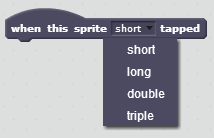
\includegraphics{images/When_This_Sprite_Is_Tapped.PNG}
\caption{The ``when this sprite is tapped" block expanded to demonstrate some of the simple gestures that could easily be supported.}
\end{figure}

\section{Evaluation}
Following intuition, the simplicity of the Closest Finger Design makes the simple low floor case projects easy to implement, but makes some of the harder case projects literally impossible to implement. While it is obvious that the Closest Finger Design simplifies the handling of single-touch inputs, surprisingly, a few common multi-touch interactions are also easy to implement using the design.

\subsection{Low Floor}
Due in part to the assumption of the existence of at most one touch on the tablet at a time, the Closest Finger Design excels with the low floor case projects. 

For example, the controls of the one-player Pong game can easily be implemented by constantly updating the x-coordinate of the paddle to the value of ``finger x". In the beginning of each game, the paddle's x-coordinate will first be mapped to $0$ (the arbitrary default value of ``finger x" before any touches have been made). After the first touch has been made, the paddle will follow the x-coordinate of the touching finger and will remain at its last location whenever the finger is lifted.

\begin{figure}
\centering
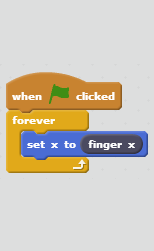
\includegraphics{images/OnePlayerPongCFD.PNG}
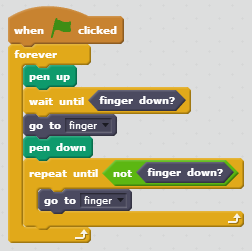
\includegraphics{images/OneFingerPaintingCFD.PNG}
\caption{On the left is an example of how the controls for one-player Pong could be implemented using the Closest Finger Design. On the right is an example script using the Closest Finger Design to program the paintbrush sprite in one-finger painting.}
\end{figure}

Implementing the controls for the one-finger painting project is a little more complicated, but is still straightforward and definitely within the capabilities of a novice Scratcher. Essentially, all the Scratcher must do is program the paint-brush to first wait for a touch to be made, then go to the touch's location and with its pen down continue following the touch until the finger is lifted. The Closest Finger Design, along with the additional framework blocks, makes programming this script almost as easy as just listing the instructions out in plain English (or any other of the sixty-six languages Scratch supports).

Recall that both of the low floor case projects were notable because they were the only two I presented that could be implemented in Desktop Scratch using mouse controls. As the result of the design's direct mapping with the Desktop Scratch mouse interaction set, many mouse-controlled Desktop Scratch projects can be directly translated into equivalent touch-controlled Tablet Scratch projects. This feature is of particular interest, because it may later become desirable for projects to be transferable between the desktop and tablet versions of Scratch.

\subsection{Middle Height}

Although both middle height case projects feature two sprites being controlled with to up-to-two simultaneous touches, one of the two project demonstrates the Closest Finger Design's greatest strength, while the other highlights its worst flaw. The two-player Pong game is well suited for this design, because the two paddles must each be programmed to follow the touch that is within their respective control ranges. On the other hand, the two paintbrush sprites in the two-finger painting project must be programmed to distribute themselves among up-to-two touches, a task that is all but impossible to program using the Closest Finger Design.

The controls for the basic two-player Pong game are extremely similar to that of the one-player Pong game when using the Closest Finger Design. In order to implement the interaction, each paddle can easily be programmed to constantly check to see if the value of ``distance to touch" is within the control range and, if that is the case, move the paddle vertically to the coordinate value ``finger y". 

\begin{figure}
\centering
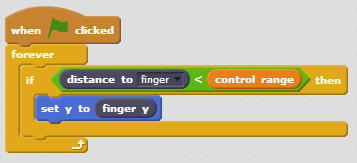
\includegraphics{images/BasicTwoPlayerPongCFD.PNG}
\caption{Here is an example script for the controlling the paddle in a basic two-player Pong game using the Closest Finger Design.}
\end{figure}

Even though each sprite can only listen to the touch nearest to themselves, many multi-touch interactions are still possible to implement. For example, it would also be simple to implement a multi-touch keyboard that allows multi-note chords to be played, just by programming each key to play its note when touched. The important factor in these implementable multi-touch interactions is that each sprite is only concerned with its closest touch, which makes the design's touch restriction advantageous rather than detrimental.

Despite the ease of implementing the basic two-player Pong game, it is terribly difficult to code the two-finger painting project using the Closest Finger Design. The main obstacle for this implementation is that each paintbrush sprite can only see the touch closest it to itself, even though it ,ay be necessary for one of the paintbrush sprites to follow the touch furthest from itself. 

One might think to first try to program the paintbrush to only follow its closest touch if the other paintbrush is not following it, but there are two significant problems with this approach. First, touches in the Closest Finger Design have no labels, so the only way to see if two sprites are listening to the same touch would be to compare their respective ``finger x" and ``finger y" values, which is an inelegant solution. Secondly, and more importantly, each paintbrush can only see the touch nearest to itself, so even if one paintbrush sprite realizes that its closest touch is already followed, it would not know where to go to find the other touch (if it even exists) and would thus have to travel around the stage looking for an unfollowed touch. While there may technically be an implementation of the two-finger painting project using the Closest Finger Design, that implementation would have to be so nonintuitive that it would not be worth considering for the purposes of this evaluation.

\subsection{High Ceiling}

Unfortunately, the simpleness of the Closest Finger Design makes the high ceiling projects essentially impossible to implement. Many complex multi-touch gestures simply cannot be implemented practically when each sprite can only listen to one touch. However, it is worth restating that many of the most popular tablet applications do not involve complex multi-touch gestures and those that do can often be redesigned to be functional with simpler controls.

Since the advanced two-player Pong game requires that each paddle simultaneously follow one touch while listening for subsequent touches that might initiate bump, it is strictly impossible to implement it exactly as specified using the Closest Finger Design. That being said, it would not be terribly difficult to make a functionally similar game with slightly more restricted controls using this interaction set. 

The implementation becomes significantly easier if the controls of the advanced two-player pong game are changed so that each paddle is moved by dragging and bumps are initiated by taps that are are close to, but not directly on the paddle. If this were the case, the paddle would simply be programmed to follow the closest touch only if the touch is within the bounds of the sprite (which can be checked using the ``touching finger?" block). To listen for bump initiating taps, a transparent crescent shaped bump detector sprite would then be created for each paddle. Both bump detectors would be programmed to follow their corresponding paddle. When a bump detector gets tapped, it would simply tell its corresponding paddle to initiate a bump.

\begin{figure}
\centering

\includegraphics{images/LeftBumper.PNG}
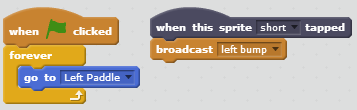
\includegraphics{images/BumperScript.PNG}
\caption{On the left is an example bump detector, colored yellow instead of transparent for visibility. On the right is the bumper detector script which programs the sprite to always follow the left paddle and to initiate a bump when tapped.}
\end{figure}

Unfortunately, the ten-finger painting project does not have a functionally equivalent alternative that is implementable with the Closest Finger Design. Since each paintbrush sprite can only see one touch and they have no practical way to distinguish which touches are not being followed, there does not exist a reasonable implementation for this project.

\section{Possible Extension}

Many of the limitations of the Closest Finger Design are the direct result of sprites only being able to listen to one touch at a time. While this restriction makes certain multi-touch interactions essentially impossible to program, it makes simple single-touch interactions very easy to program. Thus, the challenge in extending the Closest Finger Design to allow sprites to listen to multiple fingers lies in preserving the ease of programming simple touch controls.

\subsection{Specification}
The possible extension I will present is to add a new special hat block to the Closest Finger Design named ``when finger pressed". Note that the trigger for this block is different from that of the ``when this sprite is tapped" block. First, the ``when finger pressed" block is triggered by all touches, even ones whose locations are not on the sprite. Also, the ``when finger pressed" block is triggered whenever a finger first makes contact to tablet, as opposed to only being triggered by a quick tap. Furthermore, the ``when finger pressed"  block has two special properties which differentiate it from all other hat blocks.

The first special property is that the \emph{touch of interest} in the execution of a stack of blocks under a ``when finger pressed" block becomes the touch that triggered the execution of that hat block instead of just the closest touch. Before the addition of this extension, all of the five function blocks and two command blocks in the Closest Finger Design have always been solely focused on the sprite's presently closest touch. That is to say the touch of interest was always the In nearly all case with the extension, this is still true current closest touch. However, when these blocks are in a stack under a ``when finger pressed" hat, they correspond to the touch that triggered the hat as opposed to always corresponding to just the closest touch. Throughout the execution of the connected stack, the Closest Finger Design blocks will always refer to the touch that triggered the hat. If the touch that triggered the hat ends (i.e., is lifted) before the execution of the stack ends, the location of interest for all of the location related Closest Finger Design blocks becomes the last location of the triggering touch. 

This property allows sprites to listen to all touches as they are made, but only within the stack of blocks under a ``when finger pressed" block. Furthermore, the sprite loses access to the touch that triggered the ``when finger pressed" hat as soon as the connected stack has finished being executed (that is unless the touch is or becomes the sprite's closest touch). Thus, for some interactions, it will be beneficial to write the stack to continue running until the touch is lifted. However, this kind of script raises the question: what happens when a second touch is made when the stack under the ``when finger pressed" block is still executing from the first triggering? The answer to this question is the ``when finger pressed" block's second special property.

Instead of ignoring the second trigger or restarting the execution of its stack (as the other hats do), the ``when finger pressed" hat block essentially ``clones" its stack and executes it another in a thread. In each of these identical threads the touch of interest becomes the touch that triggered the making of the thread. Thus when three simultaneous touches are made, the stack connected to ``when finger pressed" block will execute three threads in parallel, each listening to a separate touch.
 
\subsection{Use Cases}

When augmented with the ``when finger pressed" hat block, the Closest Finger Design becomes powerful enough to implement the advanced two-player Pong game relatively easily . The paddles can use the ``when finger pressed" hat block to first find a touch to follow and then, when following the touch, listen for a bump initiating touch. The basic idea of the such a script is presented in Figure \ref{AdvancedTwoPlayerPongCFD}.

\begin{figure}
\centering
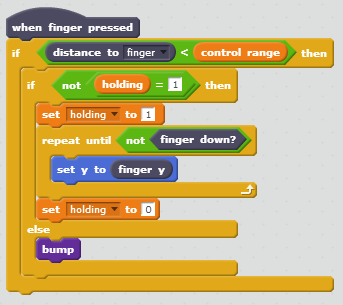
\includegraphics{images/AdvancedTwoPlayerPongCFD.PNG}
\caption{Example paddle script for advanced two-player pong using the ``when finger pressed" hat block.}
\label{AdvancedTwoPlayerPongCFD}
\end{figure}

The addition of the ``when finger pressed" block still does not make it possible to elegantly implement the multi-finger painting projects, but it does make it technically possible and significantly more practical to implement. Although all of the paintbrush sprites can listen to all of the touches with this augmentation, there still is no way to see which touches are already being followed other than the rudimentary method of checking if any of the paint brush sprites are already at the location of the touch in question. Thus, the multi-finger painting projects can be implemented by having each paintbrush use the ``when finger pressed" hat block to listen to all of the touches being made. If the paintbrush is not already following a touch, the paintbrush will follow the first incoming touch it encounters to the completion of touch if the touch is not already being followed. In figure I present the basic idea of this script.

\begin{figure}
\centering
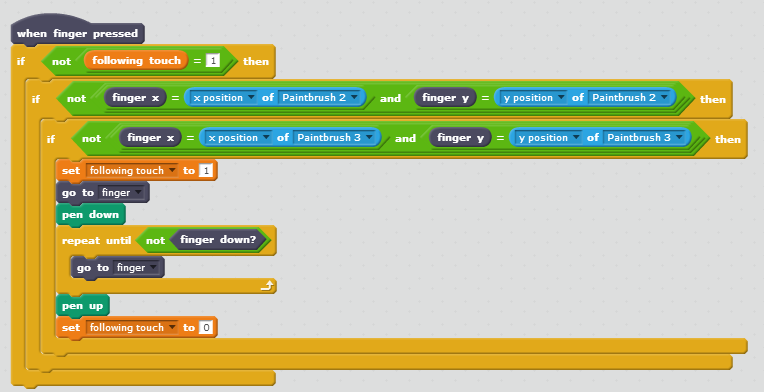
\includegraphics[width=1.0\textwidth]{images/MultiFingerPaintingCFD.PNG}
\caption{Example paintbrush script for three-finger painting using the ``when finger pressed" hat block. Note that more fingers can be supported by adding more paintbrush sprites and additional ``if checks".}
\label{MultiFingerPaintingCFD}
\end{figure}

\subsection{Potential Issues}
Although it is cause for concern that the ``when finger pressed" block's special influence on the touch blocks within its stack can be confusing to novice Scratchers, the main issues with the extension are a result of the block's thread-splitting feature.

One of Scratch's main design philosophies maintains that the execution of code should be visible. Since Scratch blocks are highlighted as they are executed, Scratchers can generally see in real time how their scripts are being executed. However, with the thread splitting, it is not clear how best to exhibit its execution when it is split into multiple threads. One idea would be to actually make copies of the stack as the threads are being created, but the tablet screen is so small that it could quickly become unwieldy when handling multiple simultaneous touches.

More importantly however, is the problem caused when a novice Scratcher innocently puts an infinite loop in the stack under a ``when finger pressed" hat block. In this case, a new, never-ending thread would be created at the initiation of every single touch. Since there is no bound on the total number of touches that can be made throughout the execution of a project, the number of threads that could be created is limitless. This potential for rapid thread propagation makes the project vulnerable to crashing from running out of computer resources without any indication to the novice Scratcher as to what is the cause. One possible solution would be to limit the number of threads to ten (since there can only be at most ten simultaneous touches), but the limit would be difficult to express visually and might restrict intentional use of the thread splitting feature.


